Workflow execution time modeling and estimation requires a methodology of 
modeling the execution time of the individual tasks of the workflow as well as 
the overheads imposed by the used middleware. As described in \S2, a task is a 
stand alone process with well defined input, output, termination criteria and 
resource requirements. Classical analysis requires to derive the complexity of 
the algorithm used either analytically or experimentally. The complexity 
function would then provide a model of the execution time of a task. That 
requires that the task's algorithm, as well as its implementation, are well 
known. 

Individual task performance on an HPC resource depends on several factors that 
are not tunable or accessible to the user, such as shared filesystem 
performance, power management policies, and selected runtime system amongst 
others. As a result, the execution time of a task may differ significantly 
between different executions. This breaks from the expectation that a complexity 
based model can provide an accurate estimate. In addition, data intensive tasks 
are highly dependent to the filesystem performance. Thus, we model the 
execution time of a task by considering the tasks as a black box. The only 
information we have prior to execution is the input of the task, for example 
input data size or other parameters.
\gpnote{Can we model the execution time of a task as a distribution whose 
expected value is modeled by the complexity of the algorithm? Makes sense and 
it might include information of }

In Ref.~\cite{paraskevakos2019workflow}, we model the execution time of a 
data-intensive workflow as a function of their input data. Our proposed 
methodology uses a linear function to model the execution time. We fitted the 
function to the data by employing a non-linear least squares algorithm and used 
$R^{2}$ and the error of the estimation as the metrics to validate our fit. 
Specifically, the workflow under investigation requires the execution of two 
tasks consecutively over a set of inputs. The tasks, $T_{1}$ and $T_{2}$, are 
heterogeneous, and have different computational requirements. 
Figure~\ref{fig:sealfitting} shows results of the fitting. In addition, based 
on the $R^{2}$ and standard error values we were able to conclude that our 
fitting produced models that explained the execution time of the tasks.

\begin{figure*}[ht!]
    \centering
    \begin{subfigure}[b]{0.45\textwidth}
        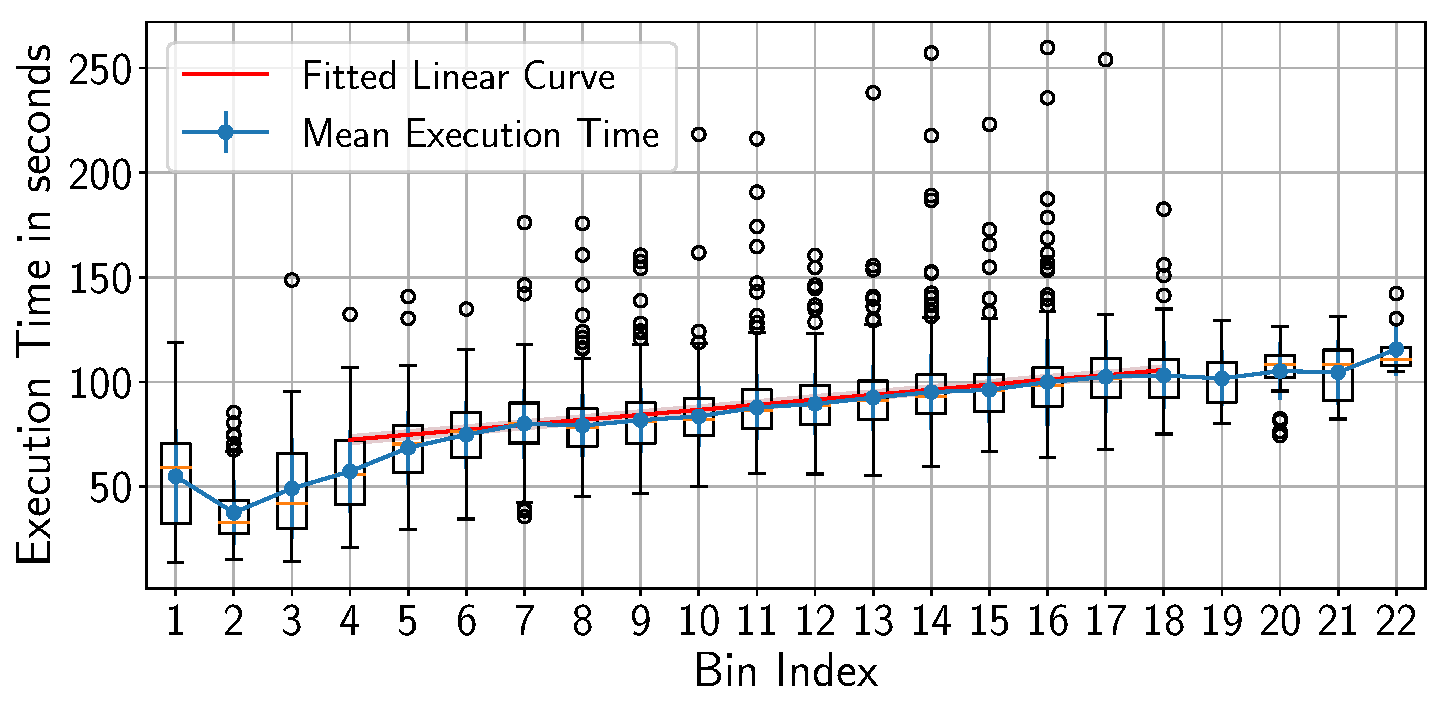
\includegraphics[width=\linewidth]{figures/stage_0_tx_box.pdf}
        \caption{Box-plots of T1 execution time, mean and STD for 125 MB image 
        size bins. Red line shows fitted linear function.}
    \end{subfigure}%
    ~ 
    \begin{subfigure}[b]{0.45\textwidth}
        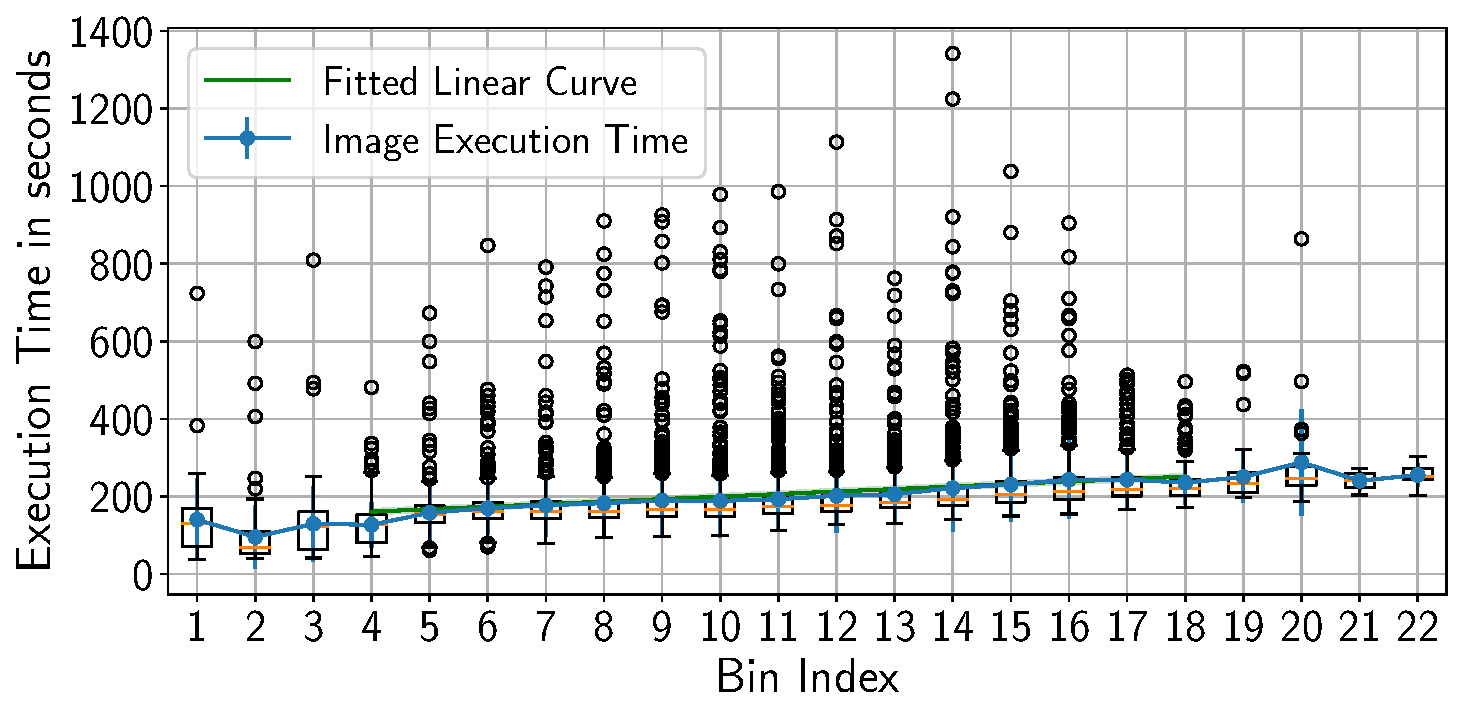
\includegraphics[width=\linewidth]{figures/stage_1_tx_box.pdf}
        \caption{Box-plots of T2 execution time, mean and STD for 125 MB image 
        size bins. Green line shows fitted linear function.}
    \end{subfigure}
    \caption{Task execution time of the tasks of a simple workflow supporting an 
    earth science use case.}
    \label{fig:sealfitting}
\end{figure*}

This works allows us to conclude that modeling the execution time of a task 
based on the initial input, with no knowledge of the specifics, provides an 
accurate estimate. This, in turn can be used to build models for the execution 
of the workflow partitions that comprise the campaign.